\documentclass[landscape]{seminar}

% You need graphics package
\usepackage{color}
\usepackage{graphicx}

\usepackage{pst-node}

\usepackage{advi}
\usepackage{advi-annot}
\usepackage{hyperref}

\usepackage{fancyheadings}

%% \usepackage[annot]{advi} 
%% must occur after packages using PStricks macros 
%% (it redefines some of them) 

\def\mathsym#1{\ifmmode{#1}\else$#1$\fi}

\pagestyle{empty}

\definecolor{c1}{rgb}{1.0,0.0,0.0}
\definecolor{c2}{rgb}{0.5,0.4,0.0}
\definecolor{c3}{rgb}{0.0,0.8,0.0}
\definecolor{c4}{rgb}{0.0,0.4,0.5}
\definecolor{c5}{rgb}{0.0,0.0,1.0}
\definecolor{c6}{rgb}{0.5,0.0,0.5}

\def\smallpause{0.2}

\def\advifooter{\vbox to 0em{\vbox to \vsize {\vfill
Press: \underline{n}ext page \underline{p}revious page
\underline{\textvisiblespace} next pause} \vss}}

\def\title#1#2{\noindent
{\bf\large #1}\\

\includegraphics[width=\textwidth]{bar.jpg.eps}
\vspace{#2cm}
}

%\let \Newpage \newpage
%\def \newpage {\Newpage \advifooter\adviheader}

\def\target#1{\hypertarget{#1}{}}


\begin{document}

\pagestyle{fancy}

%%%%%%%%%%%%%%%%%%%

\begin{slide}
\begin{center}
\vspace{0.5cm}

{\large{D\'eveloppements dans le cadre de l'ODL OCaml}}
\vspace{0.3cm}


\includegraphics[width=3cm]{logo.gif.eps}
\vspace{0.9cm}
\end{center}

\begin{enumerate}
\item \hyperlink{ocamlodbc}{OCamlODBC}
\item \hyperlink{ocamldoc}{OCamldoc}
\item \hyperlink{cameleon}{Cameleon et les cliquodromes}
\item \hyperlink{hump}{D\'emo de Cameleon sur l'outil {\tt hump}}
\end{enumerate}

\vspace{0.8cm}

\begin{flushright}

\includegraphics[width=2cm]{ocaml.eps}
\adviembed[sticky,name=clock,width=1cm,height=1cm]{../../../test/adviclock -d 50 -window !p 300 420 600 600}
\end{flushright}
\end{slide}

%%%%%%%%%%%%%%%%%%%%%%%%%%%%%%%%%%%%%%%%%%%%%

\begin{slide}
\target{ocamlodbc}
\title{OCamlODBC}{0.5}

\begin{center}
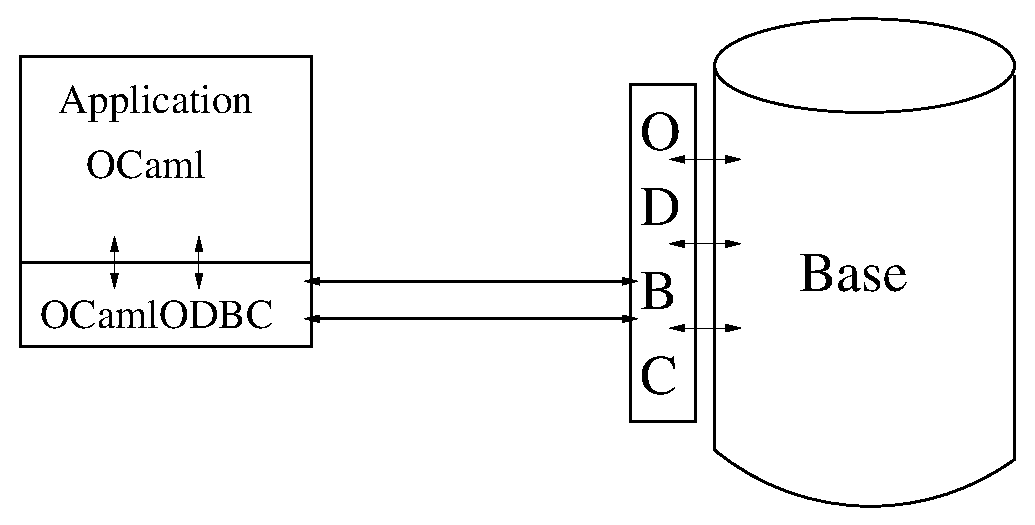
\includegraphics[width=0.8\textwidth]{ODBC.eps}
\end{center}
\end{slide}

%%%%%%%%%%%%%%%%%%%

\begin{slide}
\title{OCamlODBC - Bases support\'ees}{0.5}
\target{ocamlodbc1}
\begin{itemize}
\item MySQL
\item PostgreSQL
\item Microsoft Access
\item OpenIngres
\item DB2
\end{itemize}
+ bases support\'ees par unixODBC.

\end{slide}

%%%%%%%%%%%%%%%%%%%

\begin{slide}
\title{OCamlODBC - Interface}{0.5}
\target{ocamlodbc1}

{\tt type\hspace{0.2cm}}{\tt {\bf connection}}

{\tt val\hspace{0.2cm}{\bf connect}\hspace{0.2cm}:\hspace{0.2cm}}
{\tt string\hspace{0.2cm}$\rightarrow$\hspace{0.2cm}string\hspace{0.2cm}$\rightarrow$\hspace{0.2cm}string\hspace{0.2cm}$\rightarrow$\hspace{0.2cm}connection}

{\tt val\hspace{0.2cm}{\bf disconnect}\hspace{0.2cm}:\hspace{0.2cm}}
{\tt connection\hspace{0.2cm}$\rightarrow$\hspace{0.2cm}unit}

{\tt val\hspace{0.2cm}{\bf execute}\hspace{0.2cm}:\hspace{0.2cm}}
{\tt connection\hspace{0.2cm}$\rightarrow$\hspace{0.2cm}string\hspace{0.2cm}$\rightarrow$\hspace{0.2cm}int\hspace{0.2cm}*\hspace{0.2cm}string\hspace{0.2cm}list\hspace{0.2cm}list}

{\tt val\hspace{0.2cm}{\bf execute\_with\_info}\hspace{0.2cm}:\hspace{0.2cm}}
{\tt connection\hspace{0.2cm}$\rightarrow$}
{\tt string\hspace{0.2cm}$\rightarrow$}
{\tt int\hspace{0.2cm}*\hspace{0.2cm}(string\hspace{0.2cm}*\hspace{0.2cm}Libocaml\_odbc.sql\_column\_type)\hspace{0.2cm}list\hspace{0.2cm}*\hspace{0.2cm}string\hspace{0.2cm}list\hspace{0.2cm}list}

\end{slide}

%%%%%%%%%%%%%%%%%%%%%%%%%%%%%%%%%%%%%%%%%%%%%

\begin{slide}
\title{Outil de documentation~: OCamldoc}{0.5}
\target{ocamldoc}

\advikillembed[SIGUSR1]{clock}
\begin{itemize}
\item \hyperlink{odoc1}{architecture}
\item \hyperlink{odoc2}{syntaxe des commentaires}
\end{itemize}
\end{slide}

%%%%%%%%%%%%%%%%%%%

\begin{slide}
%\title{OCamldoc - Architecture}{0.2}
\target{odoc1}

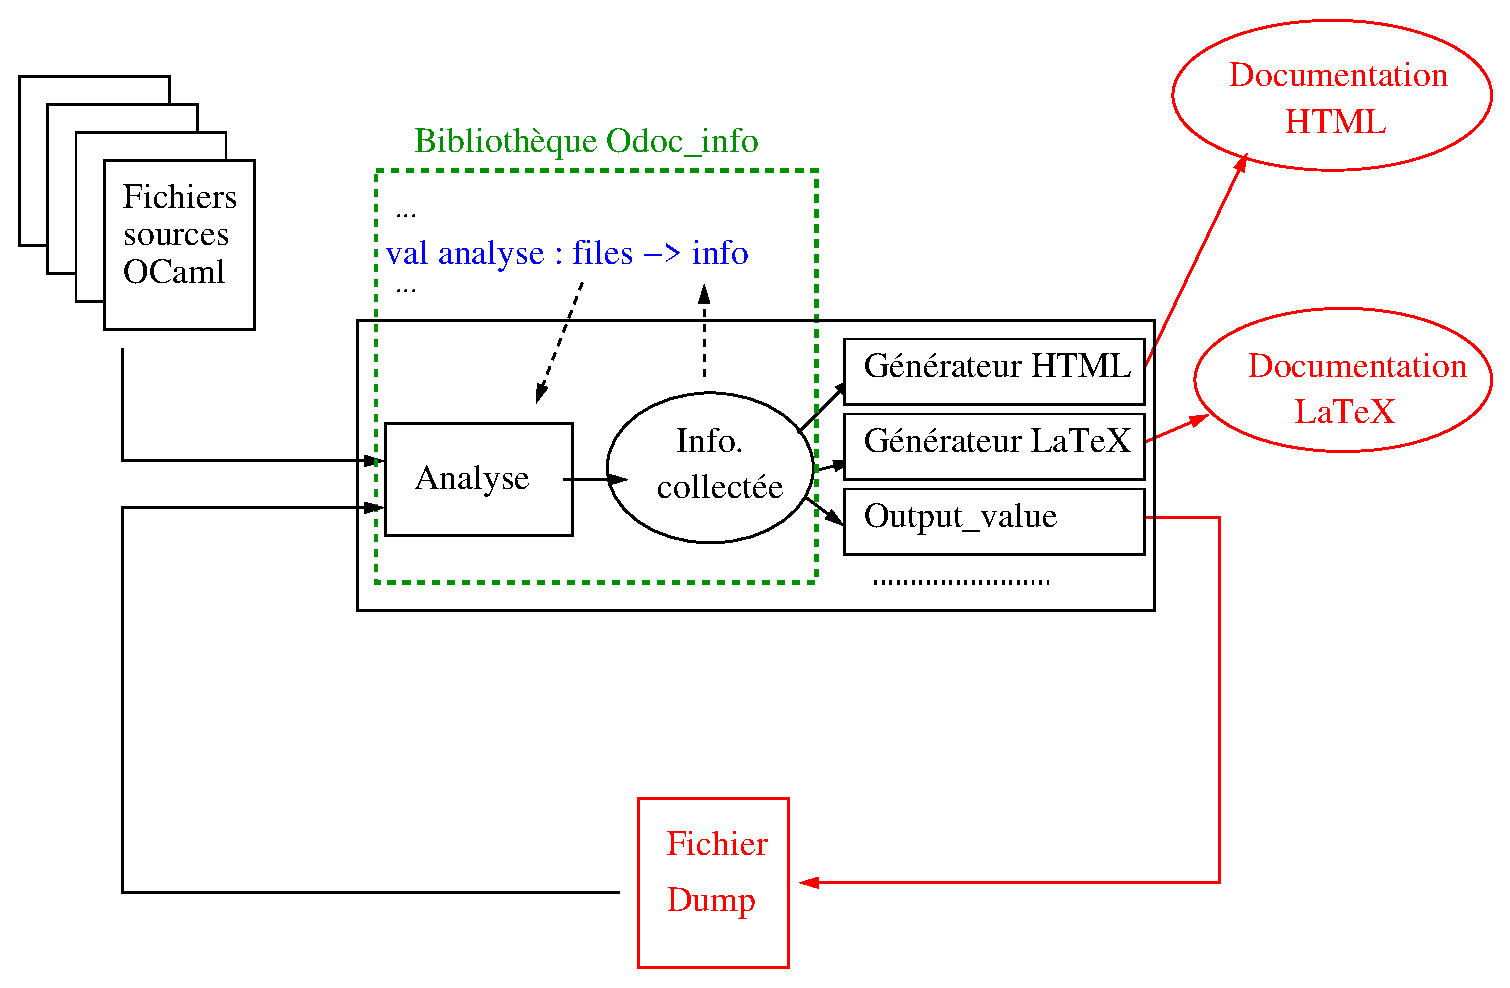
\includegraphics[width=\textwidth]{ocamldoc.eps}
\end{slide}

%%%%%%%%%%%%%%%%%%%

\begin{slide}
\title{OCamldoc - Syntaxe des commentaires}{0}
\target{odoc2}
{\scriptsize {\begin{verbatim}
(** Un <I>commentaire</I> se compose d'une partie {i texte} 
  et d'une partie ``a la Javadoc''.
@param x explication du parametre x.
@param y explication du parametre y.
@raise Failure quand on echoue.
@deprecated indique que l'element ne doit plus etre utilise
@author Lucky Luke
@author Jessie James
@since 1887
@version 1.2.3
@see <http://www.inria.fr> le site de l'inria
@see 'doc/spec.txt' pour plus d'information
@see ``OCaml reference manual'' pour plus d'information
@return l'age du capitaine
*)
\end{verbatim}
}}
\end{slide}

%%%%%%%%%%%%%%%%%%%%%%%%%%%%%%%%%%%%%%%%%%%%%

\begin{slide}
\title{Cameleon et les cliquodromes}{0.5}
\target{cameleon}

\advikillembed[SIGUSR1]{clock}
Cameleon =
\begin{quote}
 OCamlCVS \\
 + DBForge\\
 + Report\\
 + Zoggy\\
 + OCamldoc et butineur de documentation\\
 + interface avec Emacs, EFuns, XEmacs.
\end{quote}
\end{slide}


%%%%%%%%%%%%%%%%%%%
\begin{slide}
%\title{Cameleon(2)}{0.0}
\target{cam2}
%\begin{center}
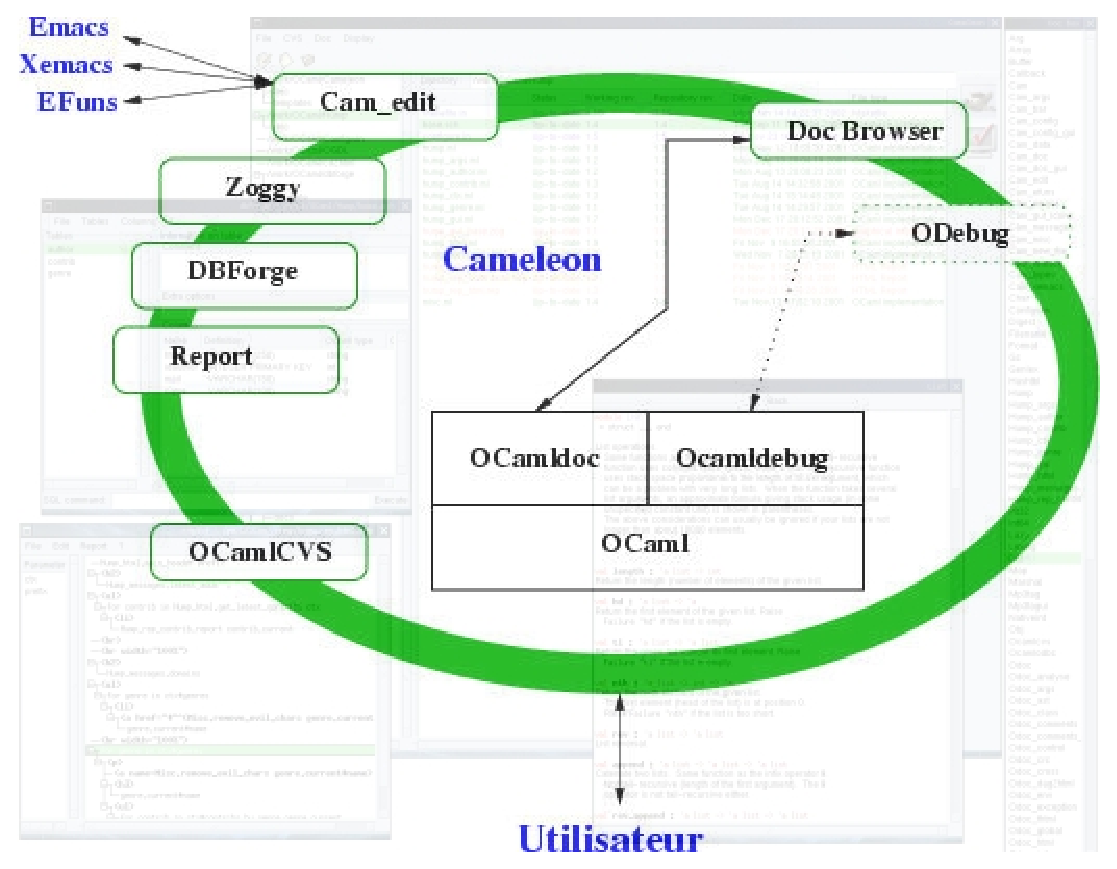
\includegraphics[width=0.95\textwidth]{cameleon.eps}
%\end{center}	

\end{slide}

%%%%%%%%%%%%%%%%%%%
\begin{slide}
%\title{Cameleon(3)}{0.0}
\target{cam3}
%\begin{center}
\includegraphics[width=0.95\textwidth]{cameleon2.eps}
%\end{center}	

\end{slide}


%%%%%%%%%%%%%%%%%%%%%%%%%%%%%%%%%%%%%%%%%%%%%

\begin{slide}
\title{Utilisation de Cameleon pour {\tt hump}}{0.0}
\target{hump}

\advikillembed[SIGUSR1]{clock}
\begin{center}
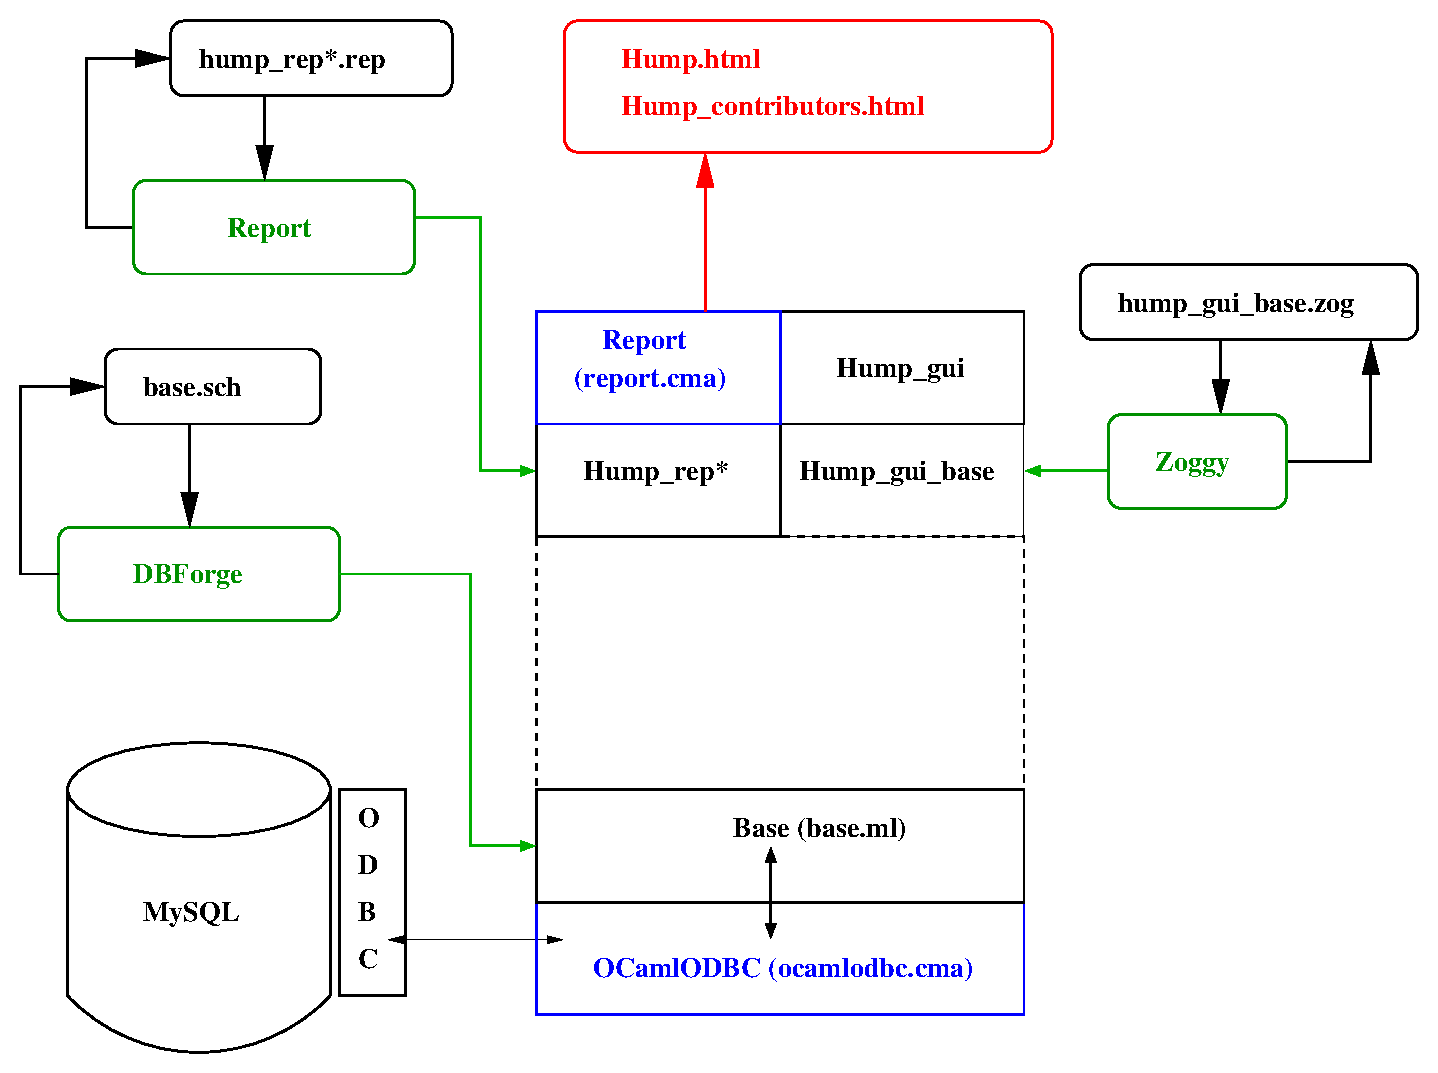
\includegraphics[width=\textwidth]{hump.eps}
\end{center}	

\end{slide}

\end{document}
